\mbox{$\displaystyle $\,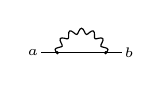
\begin{tikzpicture}[x=0.340cm, y=0.340cm, line width=0.420pt, baseline={([yshift=-0.6ex]0,0)}]
  \draw (-0.900,0.000) -- (0.900,0.000);
  \draw plot[smooth, tension=0.7] coordinates {(-0.900,0.000) (-0.967,0.063) (-0.987,0.124) (-0.943,0.170) (-0.856,0.199) (-0.769,0.218) (-0.722,0.248) (-0.728,0.303) (-0.769,0.383) (-0.802,0.468) (-0.793,0.532) (-0.733,0.555) (-0.642,0.543) (-0.555,0.522) (-0.500,0.528) (-0.482,0.580) (-0.484,0.670) (-0.476,0.762) (-0.441,0.815) (-0.377,0.810) (-0.300,0.759) (-0.231,0.702) (-0.179,0.684) (-0.140,0.723) (-0.102,0.804) (-0.055,0.883) (0.000,0.916) (0.055,0.883) (0.102,0.804) (0.140,0.723) (0.179,0.684) (0.231,0.702) (0.300,0.759) (0.377,0.810) (0.441,0.815) (0.476,0.762) (0.484,0.670) (0.482,0.580) (0.500,0.528) (0.555,0.522) (0.642,0.543) (0.733,0.555) (0.793,0.532) (0.802,0.468) (0.769,0.383) (0.728,0.303) (0.722,0.248) (0.769,0.218) (0.856,0.199) (0.943,0.170) (0.987,0.124) (0.967,0.063) (0.900,0.000)};
  \draw (-0.900,0.000) -- (-1.500,0.000);
  \draw (0.900,0.000) -- (1.500,0.000);
  \fill (-0.900,0.000) circle (0.064);
  \fill (0.900,0.000) circle (0.064);
  \node[font=\tiny, inner sep=0pt, anchor=0] at (-1.590,0.000) {$a$};
  \node[font=\tiny, inner sep=0pt, anchor=180] at (1.590,0.000) {$b$};
\end{tikzpicture}}
